\documentclass{article}
\usepackage{tikz}

\begin{document}

\begin{figure}[h]
    \centering
    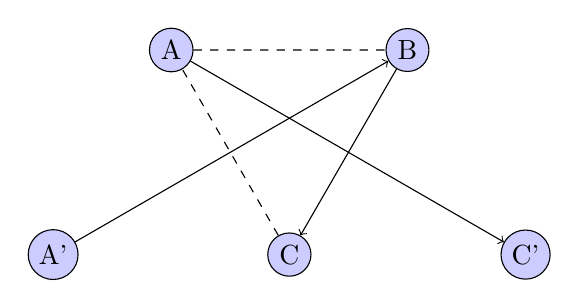
\begin{tikzpicture}[scale=1.5, every node/.style={circle, draw, fill=blue!20, inner sep=2pt}]
        % Nodes
        \node (A) at (0,0) {A};
        \node (B) at (2,0) {B};
        \node (C) at (1,-1.732) {C};
        \node (A') at (-1,-1.732) {A'};
        \node (C') at (3,-1.732) {C'};

        % Edges
        \draw[->] (A) -- (C');
        \draw[->] (B) -- (C);
        \draw[->] (A') -- (B);

        % Internal 3-cycle
        \draw[dashed, ->] (C) -- (A) -- (B) -- cycle;
    \end{tikzpicture}
    \caption{Eulerian Circuit with Given Connections}
\end{figure}

\end{document}